\documentclass[11pt]{article}
\usepackage[textwidth=18.0cm, textheight=23.0cm, top=2.0cm]{geometry}
\usepackage{pst-all}
\usepackage{amssymb}
\usepackage{tikz}
\usepackage{underscore}\begin{document}
\pagestyle{empty}


ClassName: \underline{\textbf{Class_04.2bp-15}}
\par
BinSize: \underline{\textbf{100 × 100}}
\par
ReduceSize: \underline{\textbf{100 × 100}}
\par
TypeNum: \underline{\textbf{38}}
\par
Num: \underline{\textbf{40}}
\par
OutS: \underline{\textbf{20000}}
\par
InS: \underline{\textbf{11156}}
\par
Rate: \underline{\textbf{0.558}}
\par
UB: \underline{\textbf{2}}
\par
LB0: \underline{\textbf{2}}
\par
LB: \underline{\textbf{2}}
\par
LBWithCut: \underline{\textbf{2}}
\par
NodeCut: \underline{\textbf{0}}
\par
ExtendedNodeCnt: \underline{\textbf{1}}
\par
GenNodeCnt: \underline{\textbf{1}}
\par
PrimalNode: \underline{\textbf{0}}
\par
ColumnCount: \underline{\textbf{2}}
\par
TotalCutCount: \underline{\textbf{0}}
\par
RootCutCount: \underline{\textbf{0}}
\par
LPSolverCnt: \underline{\textbf{1}}
\par
PricingSolverCnt: \underline{\textbf{0}}
\par
BranchAndBoundNum: \underline{\textbf{1}}
\par
isOpt: \underline{\textbf{true}}
\par
TimeOnInitSolution: \underline{\textbf{0.000 s}}
\par
TimeOnPrimal: \underline{\textbf{0.000 s}}
\par
TimeOnPricing: \underline{\textbf{0.000 s}}
\par
TimeOnRmp: \underline{\textbf{0.065 s}}
\par
TotalTime: \underline{\textbf{0.149 s}}
\par
\newpage


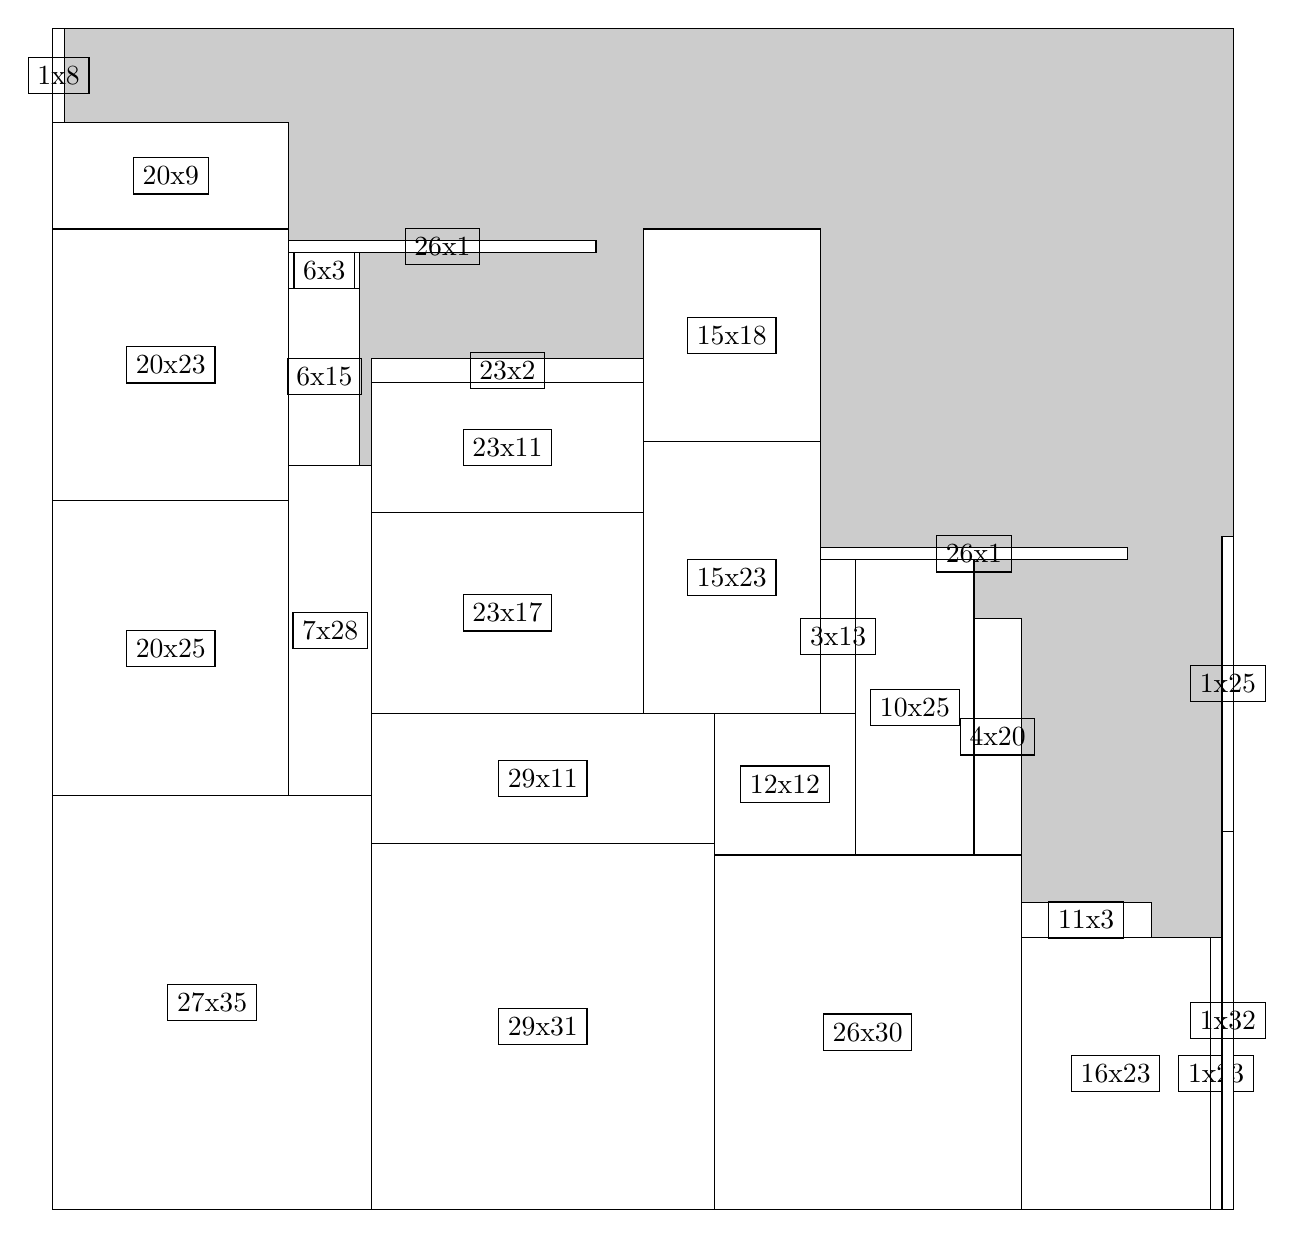
\begin{tikzpicture}[shorten >=1pt,scale=1.0,every node/.style={scale=1.0},->]
\tikzstyle{vertex}=[circle,fill=black!25,minimum size=14pt,inner sep=0pt]
\filldraw[fill=gray!40!white, draw=black] (0,0) rectangle (15.0,15.0);
\foreach \name/\x/\y/\w/\h in {27x35/0.0/0.0/4.05/5.25,29x31/4.05/0.0/4.35/4.6499999999999995,26x30/8.4/0.0/3.9/4.5,20x25/0.0/5.25/3.0/3.75,20x23/0.0/9.0/3.0/3.4499999999999997,23x17/4.05/6.3/3.4499999999999997/2.55,16x23/12.299999999999999/0.0/2.4/3.4499999999999997,15x23/7.5/6.3/2.25/3.4499999999999997,29x11/4.05/4.6499999999999995/4.35/1.65,15x18/7.5/9.75/2.25/2.6999999999999997,23x11/4.05/8.85/3.4499999999999997/1.65,10x25/10.2/4.5/1.5/3.75,7x28/3.0/5.25/1.05/4.2,20x9/0.0/12.45/3.0/1.3499999999999999,12x12/8.4/4.5/1.7999999999999998/1.7999999999999998,1x23/14.7/0.0/0.15/3.4499999999999997,4x20/11.7/4.5/0.6/3.0,23x2/4.05/10.5/3.4499999999999997/0.3,3x13/9.75/6.3/0.44999999999999996/1.95,11x3/12.299999999999999/3.4499999999999997/1.65/0.44999999999999996,1x32/14.85/0.0/0.15/4.8,26x1/9.75/8.25/3.9/0.15,26x1/3.0/12.15/3.9/0.15,1x25/14.85/4.8/0.15/3.75,6x15/3.0/9.45/0.8999999999999999/2.25,6x3/3.0/11.7/0.8999999999999999/0.44999999999999996,1x8/0.0/13.799999999999999/0.15/1.2}
\filldraw[fill=white!40!white, draw=black] (\x,\y) rectangle node[draw] (\name) {\name} ++(\w,\h);
\end{tikzpicture}


w =27 , h =35 , x =0 , y =0 , v =945
\par
w =29 , h =31 , x =27 , y =0 , v =899
\par
w =26 , h =30 , x =56 , y =0 , v =780
\par
w =20 , h =25 , x =0 , y =35 , v =500
\par
w =20 , h =23 , x =0 , y =60 , v =460
\par
w =23 , h =17 , x =27 , y =42 , v =391
\par
w =16 , h =23 , x =82 , y =0 , v =368
\par
w =15 , h =23 , x =50 , y =42 , v =345
\par
w =29 , h =11 , x =27 , y =31 , v =319
\par
w =15 , h =18 , x =50 , y =65 , v =270
\par
w =23 , h =11 , x =27 , y =59 , v =253
\par
w =10 , h =25 , x =68 , y =30 , v =250
\par
w =7 , h =28 , x =20 , y =35 , v =196
\par
w =20 , h =9 , x =0 , y =83 , v =180
\par
w =12 , h =12 , x =56 , y =30 , v =144
\par
w =1 , h =23 , x =98 , y =0 , v =23
\par
w =4 , h =20 , x =78 , y =30 , v =80
\par
w =23 , h =2 , x =27 , y =70 , v =46
\par
w =3 , h =13 , x =65 , y =42 , v =39
\par
w =11 , h =3 , x =82 , y =23 , v =33
\par
w =1 , h =32 , x =99 , y =0 , v =32
\par
w =26 , h =1 , x =65 , y =55 , v =26
\par
w =26 , h =1 , x =20 , y =81 , v =26
\par
w =1 , h =25 , x =99 , y =32 , v =25
\par
w =6 , h =15 , x =20 , y =63 , v =90
\par
w =6 , h =3 , x =20 , y =78 , v =18
\par
w =1 , h =8 , x =0 , y =92 , v =8
\par
\newpage


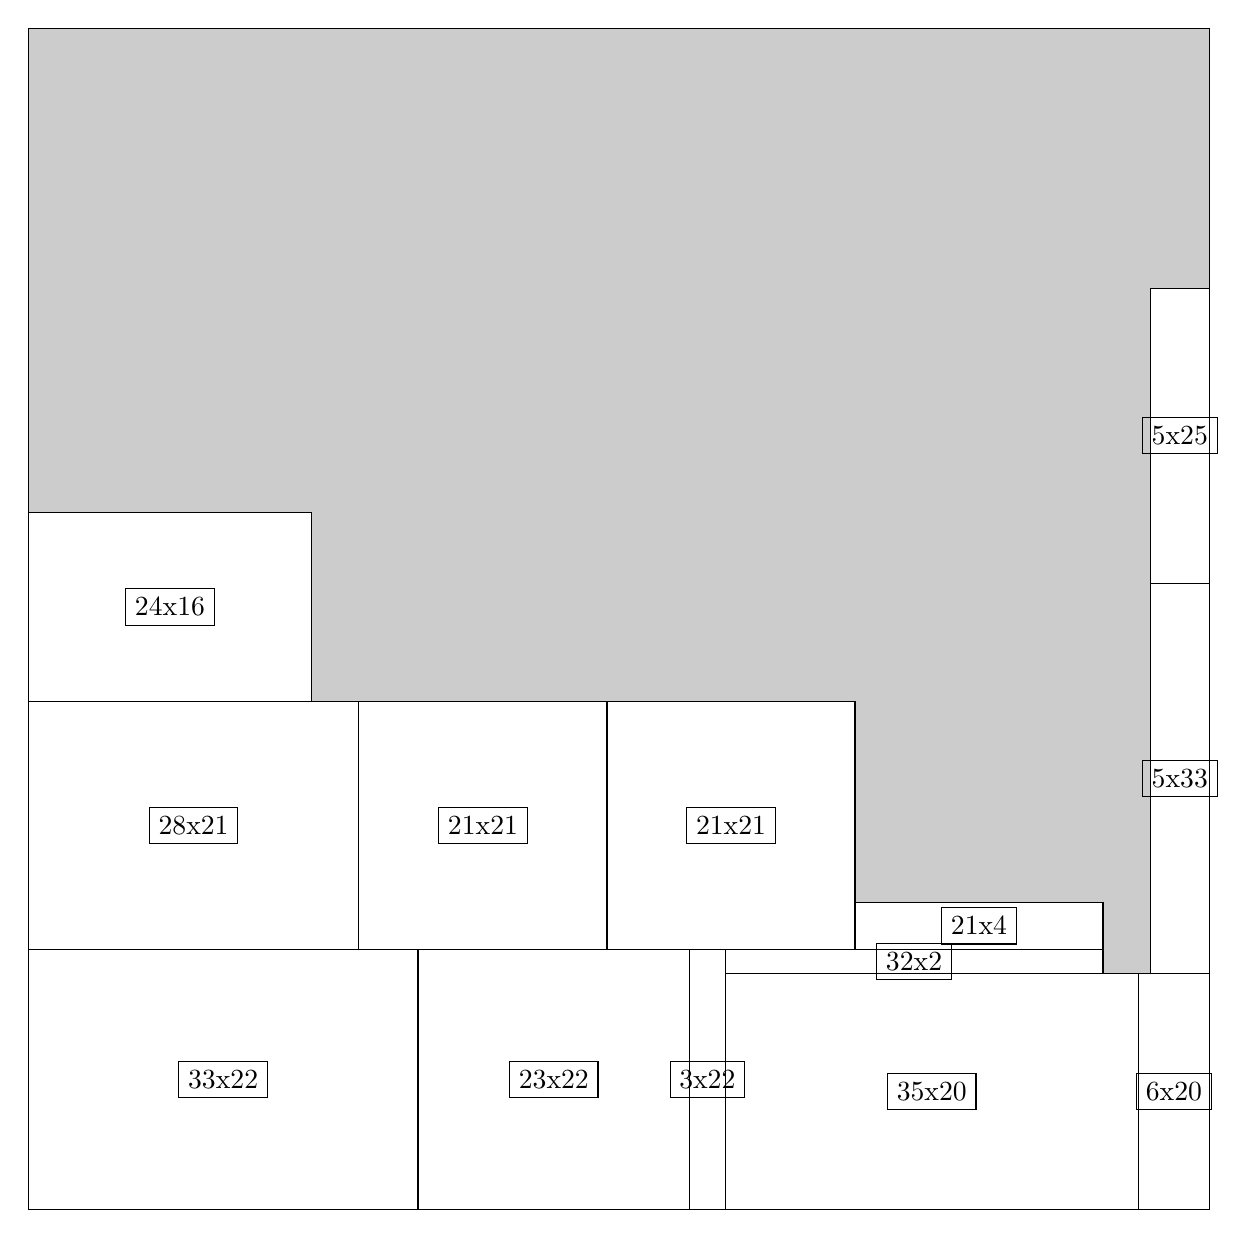
\begin{tikzpicture}[shorten >=1pt,scale=1.0,every node/.style={scale=1.0},->]
\tikzstyle{vertex}=[circle,fill=black!25,minimum size=14pt,inner sep=0pt]
\filldraw[fill=gray!40!white, draw=black] (0,0) rectangle (15.0,15.0);
\foreach \name/\x/\y/\w/\h in {33x22/0.0/0.0/4.95/3.3,35x20/8.85/0.0/5.25/3.0,28x21/0.0/3.3/4.2/3.15,23x22/4.95/0.0/3.4499999999999997/3.3,21x21/4.2/3.3/3.15/3.15,21x21/7.35/3.3/3.15/3.15,24x16/0.0/6.45/3.5999999999999996/2.4,5x33/14.25/3.0/0.75/4.95,5x25/14.25/7.949999999999999/0.75/3.75,6x20/14.1/0.0/0.8999999999999999/3.0,21x4/10.5/3.3/3.15/0.6,3x22/8.4/0.0/0.44999999999999996/3.3,32x2/8.85/3.0/4.8/0.3}
\filldraw[fill=white!40!white, draw=black] (\x,\y) rectangle node[draw] (\name) {\name} ++(\w,\h);
\end{tikzpicture}


w =33 , h =22 , x =0 , y =0 , v =726
\par
w =35 , h =20 , x =59 , y =0 , v =700
\par
w =28 , h =21 , x =0 , y =22 , v =588
\par
w =23 , h =22 , x =33 , y =0 , v =506
\par
w =21 , h =21 , x =28 , y =22 , v =441
\par
w =21 , h =21 , x =49 , y =22 , v =441
\par
w =24 , h =16 , x =0 , y =43 , v =384
\par
w =5 , h =33 , x =95 , y =20 , v =165
\par
w =5 , h =25 , x =95 , y =53 , v =125
\par
w =6 , h =20 , x =94 , y =0 , v =120
\par
w =21 , h =4 , x =70 , y =22 , v =84
\par
w =3 , h =22 , x =56 , y =0 , v =66
\par
w =32 , h =2 , x =59 , y =20 , v =64
\par
\newpage


\end{document}